\documentclass[12pt]{article}
\usepackage{tikz}
\usepackage{float}
\usepackage[utf8]{inputenc}

\begin{document}
%\oddsidemargin=-5mm \evensidemargin=-5mm \marginparwidth=.08in
%\marginparsep=.01in \marginparpush=5pt \topmargin=-15mm
%\headheight=12pt \headsep=25pt \footheight=12pt \footskip=30pt
%\textheight=25cm \textwidth=17cm \columnsep=2mm \columnseprule=1pt
%\parindent=15pt\parskip=2pt

\begin{center}
\bf Semestralní projekt MI-PPR 2015/2016:\\[5mm]
    Paralelní algoritmus pro řešení problému ZBS\\[5mm]
       Valentin Banshchikov\\
       Michal Kápar\\[2mm]
magisterské studijum, FIT ČVUT, Kolejní 550/2, 160 00 Praha 6\\[2mm]
\today
\end{center}

\section{Definice problému}
\subsection{Vstupní data}

\begin{description}
	\item[a] -- přirozené číslo,
	\item[n] -- přirozené číslo představující počet uzlů grafu G, $5 \leq n$,
	\item[m] -- přirozené číslo představující počet hran grafu G, $n \leq m$,
	\item[k] -- přirozené číslo řádu jednotek představující průměrný stupeň uzlu grafu G, $3 \leq k \leq n$,
	\item[$G(V,E)$] -- jednoduchý souvislý neorientovaný neohodnocený graf o n uzlech a m hranách.
\end{description}

\subsection{Úkol}

Naleznout rozdělení množiny n uzlů grafu G do dvou disjunktních podmnožin X a Y tak, že podmnožina X obsahuje a uzlů, podmnožina Y obsahuje $n-a$ uzlů $a$ počet všech hran $\{u,v\}$ takových, že u je z X a v je z Y, je minimální.

\subsection{Výstup algoritmu}

Výpis disjuktních množin uzlů X a Y a počet hran tyto množiny spojující.

\subsection{Popis vstupu}

Algoritmus dostává na vstup matici přechodů s číslem $a$. Matice je generována z aplikace \texttt{generator}, ta vytvoří matici na základě zadané velikosti a stupně grafu. Následně je na výsledek uplatněna aplikace \texttt{souvislost}, ta má za cíl z nesouvislého grafu vygenerovat souvislý graf.

\section{Popis sekvenčního algoritmu a jeho implementace}

Sekvenční algoritmus je typu \texttt{BB-DFS} (Branch-and-bound Depth-first search). Při hledání stavového prostoru hledáme nejmenší cenu řešení. Není možné žádné stavy vynechat. Počáteční cena je nastavena na nekonečno (přesněji \texttt{UINT\_MAX}).

Implementace je popsána v následujícím pseudokódu:
\begin{verbatim}

1. MIN_HRAN = nekonečno
2. ALL_HRAN = (1, 2, 3, ..., n)
3. Vytvoř 1. kombinace v lexikografickem pořadí a zapíš 
   do proměny COMB
4. Vytvoř doplněk a zapíš do proměny COMP: 
   COMP = ALL_HRAN \ COMB
5. Spočti počet hran mezi množinou COMB a COMP
6. Pokud je počet hran menší, než MIN_HRAN:
     MIN_HRAN = nový počet hran
7. Zapíš do COMB následující kombinace v lexikografickem pořadí: 
     Pokud taková existuje:
       GOTO 4
     Pokud taková neexistuje:
       Výsledkem je MIN_HRAN 

\end{verbatim}

Na základě objemu zvolených dat vypočteme asymptotickou složitost: 

\hspace{1cm}

$O(n)={n\choose a} \cdot ((n - a) \cdot a + 2 \cdot (n + a) - 1)$

\hspace{1cm}

${n\choose a}$ je počet kombinací v podmnožině X, pro které se hledá minimum vazeb mezi podmnožinami X a Y. Násobení $(n - a) \cdot a$ představuje hledání hrany mezi podmnožinami X a Y. $2 \cdot (n + a) - 1$ je složitost výpočtu doplňku.

\section{Popis paralelního algoritmu a jeho implementace v MPI}

Paralelní algoritmus je typu \texttt{PBB-DFS-V}. To znamená, že každý proces ví, jaká je horní mez (při startu uložena v dolní mezi) a lokálně udržuje informaci o svém dosud nejlepším řešení. Pomocí paralelní redukce se ze všech nejlepších lokálních řešení vybere globálně nejlepší.

Implementace je popsána v následujícím pseudokódu:

\begin{verbatim}

1. LOCAL_MIN_HRAN = nekonečno
2. ALL_HRAN = (1, 2, 3, ..., n)
3. Každý proces vypočte podle svého čísla první a poslední 
   kombinace a zapíše je do proměn LOCAL_COMB a LOCAL_STOP
4. Vytvoř doplněk a zapíš do proměny LOCAL_COMP: 
   LOCAL_COMP = ALL_HRAN \ LOCAL_COMB
5. Spočti počet hran mezi množinou LOCAL_COMB a LOCAL_COMP
6. Pokud je počet hran menší, než LOCAL_MIN_HRAN:
     LOCAL_MIN_HRAN = nový počet hran
7. Pokud LOCAL_COMB se rovna LOCAL_STOP:
     Čekej na ostatní procesy
   Pokud ne:
     Zapíš do LOCAL_COMB následující kombinace v lexikografickem pořadí: 
     Pokud taková existuje:
       GOTO 4
     Pokud taková neexistuje:
       Čekej na ostatní procesy
8. Pošle LOCAL_MIN_HRAN procesu 0
9. Pokud je proces 0
     Spočte globální minima a vypíše výsledek

\end{verbatim}

Ideální čas výpočtu je následující:

\hspace{1cm}

$T(n,p)_{vyp} = \frac{{n \choose a}}{p}\cdot ((n - a) \cdot a + 2 \cdot (n + a) - 1)$ -- část samotného výpočtu

\hspace{1cm}

$T(n,p)_{br} = \alpha log_{2}p$-- binární redukce výsledku

\hspace{1cm}

Celkově tedy $T(n,p) = \frac{{n \choose a}}{p}\cdot ((n - a) \cdot a + 2 \cdot (n + a) - 1) + \alpha log_{2}p$

\section{Naměřené výsledky a vyhodnocení}

Pro měření byl vybrán graf o velikosti 35 vrcholů. Pro výpočet není důležité, abych byl graf řídký nebo hustý. Pro každou podmnožinu, kterých je ${n \choose a}$ se kontrolují všechny hrany. V následující tabulce jsou vyneseny rychlosti výpočtu v sekundách pro zvolenou podmnožinu grafu velikosti $a$.

\begin{table}[ht]
	\centering
	\begin{tabular}{ | l | c | c | r | }
		\hline
		 & \textbf{a=11} & \textbf{a=12} & \textbf{a=13} \\ \hline
		\textbf{1} & 251.944 & 529.863 & 967.434 \\ \hline
		\textbf{2} & 148.523 & 299.84 & 533.992 \\ \hline
		\textbf{4} & 72.56 & 152.613 & 269.537 \\ \hline
		\textbf{8} & 35.674 & 76.163 & 136.131 \\ \hline
		\textbf{12} & 24.248 & 51.47 & 90.065 \\ \hline
		\textbf{16} & 18.373 & 37.966 & 70.219 \\ \hline
		\textbf{20} & 15.129 & 30.452 & 56.116 \\ \hline
		\textbf{24} & 12.267 & 25.1 & 46.577 \\ \hline
	\end{tabular}
	\caption{Tabulka naměřených hodnot v sekundách pro graf s počtem vrcholů 35 a rozdílné velikosti podmnožiny $a$}
   \label{fig:spe}
\end{table}

Pro porovnání, že je výpočet dostatečně náročný pro zvolená $a$, slouží následující graf, ve kterém jsou vyneseny všechny časy výpočtů.

\begin{figure}[H]
  \centering
    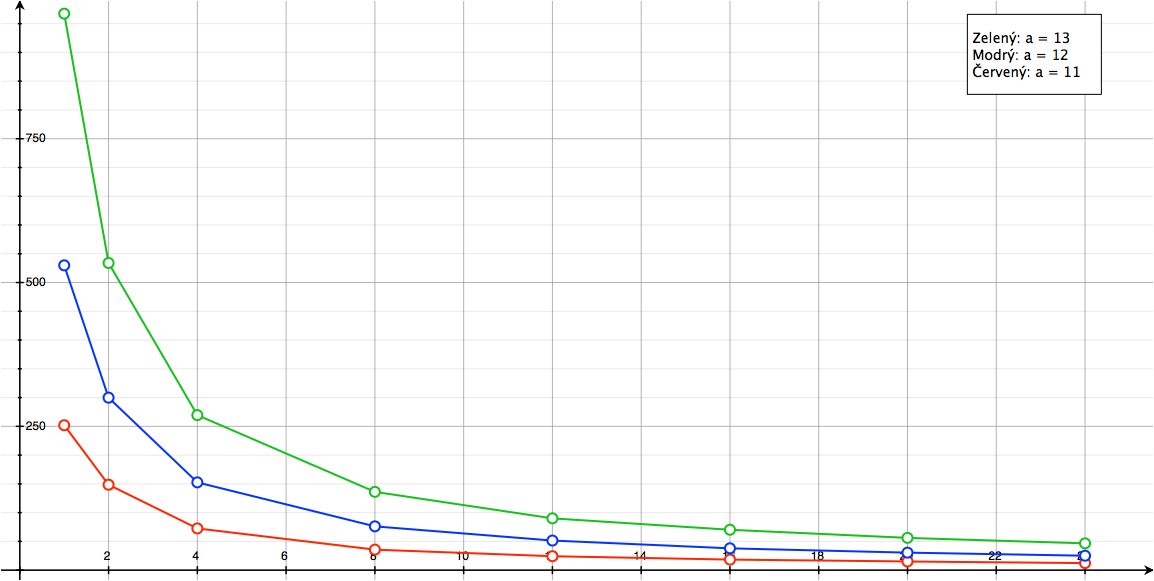
\includegraphics[width=1\textwidth]{./graph1.png}
  \caption{Graf všech výpočtů}
  \label{fig:con}
\end{figure}

\begin{figure}[H]
  \centering
    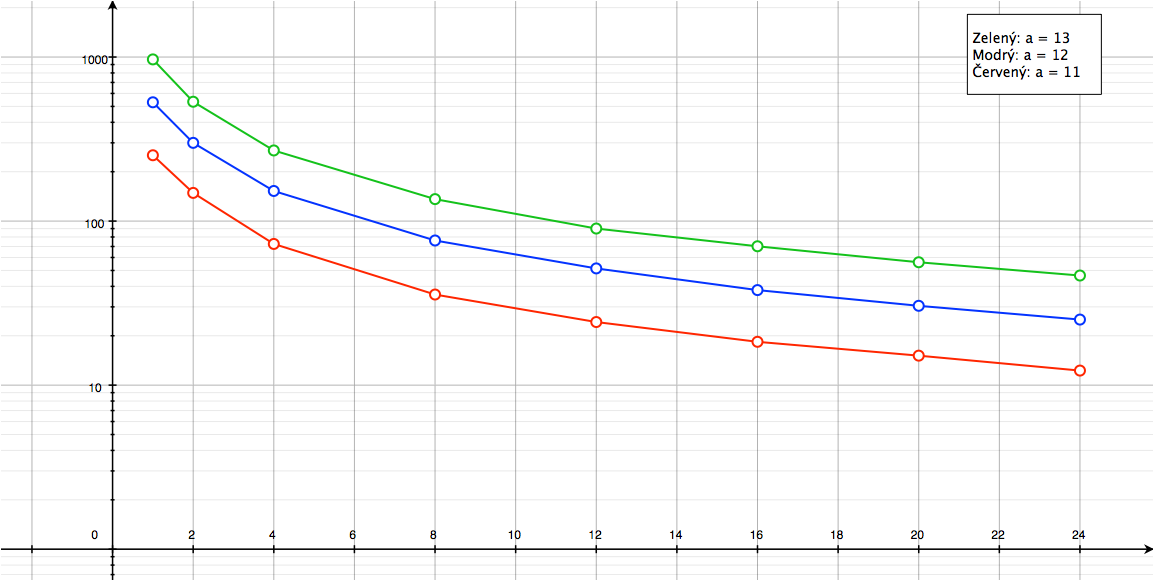
\includegraphics[width=1\textwidth]{./graph1_log.png}
  \caption{Graf všech výpočtů kde osa $y$ je logaritmická}
  \label{fig:con}
\end{figure}

\newpage
\section{Závěr}

V semestrální práci jsme si vyzkoušeli programování složitější úlohy, která lze paralelizovat k tomu jsme využili knihovnu MPI. K řešení úlohy jsme využívali výpočetní cluster STAR, propojený přes Ethernet s maximem 24 procesorů. Při zvyšování procesorů jsme se dostali k linearnímu zrychlení, které jsme podle typu úlohy a implementace našeho algoritmu čekali. 

V semestru jsme si vyzkoušeli analyzovat a navrhovat jak rešit úlohy s využitím více procesorů, přes počáteční přerozdělení problému, následnou komunikaci a výpočet na jednotlivých procesorech až po zavěrečný sběr výsledků. 

\end{document}
